\documentclass[a4,center,fleqn]{NAR}

\usepackage{lmodern}

% Enter dates of publication
\copyrightyear{2018}
\pubdate{?? ?????? ????}
\pubyear{????}
\jvolume{??}
\jissue{??}

%\articlesubtype{This is the article type (optional)}

\newcommand{\ca}{$\alpha$-carbon\xspace}
\newcommand{\cas}{$\alpha$-carbons\xspace}

\begin{document}

\title{Article title}

\author{%
Corresponding Author\,$^{1,*}$,
First Co-Author\,$^{2}$
and Second Co-Author\,$^2$%
\footnote{To whom correspondence should be addressed.
Tel: +44 000 0000000; Fax: +44 000 0000000; Email: xxx@yyyy.ac.zz}}

\address{%
$^{1}$Affiliation of Corresponding Author
and
$^{2}$Affiliation of Both Co-Authors}
% Affiliation must include:
% Department name, institution name, full road and district address,
% state, Zip or postal code, country

\history{%
Received ?????? ??, ????;
Revised ?????? ??, ????;
Accepted ?????? ??, ????}

\maketitle

\begin{abstract}
Text. Text. Text. Text. Text. Text. Text. Text. Text. Text. Text.
Text. Text. Text. Text. Text. Text. Text. Text. Text. Text. Text.
Text. Text. Text. Text. Text. Text. Text. Text. Text. Text. Text.
Text. Text. Text. Text. Text. Text. Text. Text. Text. Text. Text.
Text. Text. Text. Text. Text. Text. Text. Text. Text. Text. Text.
Text. Text. Text. Text. Text. Text. Text. Text. Text. Text. Text.
Text. Text. Text. Text. Text. Text. Text. Text. Text. Text. Text.
Text. Text. Text. Text. Text. Text. Text. Text. Text. Text. Text.
Text. Text. Text. Text. Text. Text. Text. Text. Text. Text. Text.
Text. Text. Text. Text. Text. Text. Text. Text. Text. Text. Text.
Text. Text. Text. Text. Text. Text. Text. Text. Text. Text. Text.
Text. Text. Text. Text. Text. Text. Text. Text. Text. Text. Text.
Text. Text. Text. Text. Text. Text. Text. Text. Text. Text. Text.
Text. Text. Text. Text. Text. Text. Text. Text. Text. Text. Text.
Text. Text. Text. Text. Text. Text. Text. Text. Text. Text. Text.
Text. Text. Text. Text. Text. Text. Text. Text. Text. Text. Text.
Text. Text. Text. Text. Text. Text. Text. Text. Text. Text. Text.
Text. Text. Text. Text. Text. Text. Text. Text. Text. Text. Text.
Text. Text. Text. Text. Text. Text. Text. Text. Text. Text. Text.
Text. Text. Text. Text. Text. Text. Text. Text. Text. Text. Text.
Text. Text. Text. Text. Text. Text. Text. Text. Text. Text. Text.
Text. Text. Text. Text. Text. Text. Text. Text. Text. Text. Text.
Text. Text. Text. Text. Text. Text. Text. Text. Text. Text. Text.
Text. Text.
\end{abstract}

\section{Introduction}

Proteins represent the functional end-product within the central dogma of molecular biology \citep{Crick1970}.
As such, understanding protein structure is a central goal within structural bioinformatics. 
Protein structure determination, prediction, alignment, and search all serve to advance this understanding. 
Below, we present our new approach to a fast, scalable, and purely geometric protein structure search we refer to with the cumbersome but catchy acronym of \emph{RUn Position Encoded Encodings} of residue descriptors (RUPEE).

For comparisons, we examine results from the CATHEDRAL structural scan \citep{Redfern2007} available at the CATH website \citep{Sillitoe2015}.
In addition to recognizing domains in multidomain proteins, CATHEDRAL also can be used to find structural neighbors among CATH domains for an uploaded protein data bank (PDB) file, that is, where an identifier is not provided that can be used for retrieval of pre-calculated results. 
CATHEDRAL is effective at this task but can take upwards of 10 minutes to produce results against CATH s35 representatives.

Restricting our initial approach to protein domains, we have indexed CATH v4.1 domains, consisting of 308,999 structures, and developed a feature similar to CATHEDRAL that performs a protein structure search based on a PDB file, returning results in seconds rather than minutes.
To evaluate RUPEE, we have made comparisons to the output of CATHEDRAL along two dimensions, quality of results and response times. 
In both cases, RUPEE performs better on average for the domains we evaluated. 

Besides our approach to protein structure search, we introduce a polar plot for torsion angles that may have wider applicability in the study of protein structure. 
Further, the \emph{run position encoding} heuristic introduced below may have wider applicability to algorithms for character sequences containing long runs of repeats. 

For the remainder of this paper, we first discuss some related work to provide context for our approach followed by a description of our method. 
We end with the results of evaluation with CATHEDRAL along with an analysis and conclusion. 

% **************************************************************
% Keep this command to avoid text of first page running into the
% first page footnotes
\enlargethispage{-65.1pt}
% **************************************************************

\section{METHODS}

Broadly, we define a linear encoding of protein structure and convert this linear encoding into a bag of features amenable to big data processing.
Protein structure searches that use linear encodings are not unique \citep{Carpentier2005,Daniluk2011,Ritchie2012}.
The novelty of our approach lies in its remarkable performance given its simplicity. 
Additionally, elements of our approach can be isolated and found to be useful in their own right. 

\subsection{Regions of Torsion Angles}

\begin{figure}[t]
\begin{center}
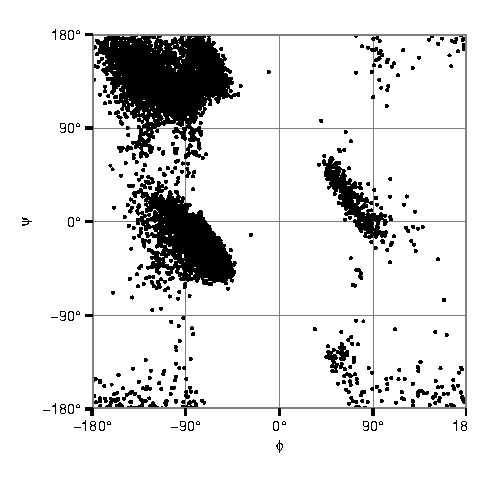
\includegraphics{ramachandran}
\end{center}
\caption{Ramachandran plot of randomly sampled torsion angles}
\label{fig:ramachandran}
\end{figure}

Our first step towards a linear encoding of protein structure is to identify separable regions of permissible torsion angles,
but first we introduce a new plot of torsion angles better suited to this effort. 

Despite their utility and familiarity, Ramachandran plots \citep{Ramachandran1968} represent angular data using a square plot better suited for scalar data.
This leads to the unwieldy arrangement where the top part of the plot is continuous with the bottom and the left is continuous with the right. 

To identify regions of torsion angles, we randomly sampled 10,000 residues from high-resolution, CATH s35 representatives to account for precision and redundancy, respectively. 
A Ramachandran plot of the sampled torsions angles is shown in \figurename~\ref{fig:ramachandran}. 
As can be seen, a single cluster of residues, consisting primarily of $\beta$-strands, appears at all 4 corners of the Ramachandran plot.

This continuity problem was partially addressed in \citet{Karplus2010} using \emph{wrapped} and \emph{mirrored} plots. 
Both wrapped and mirrored plots take advantage of the sparsely populated areas of the Ramachandran plot at $\phi = 0\degree$ and $\psi = -120\degree$.
However, with larger samples of torsion angles, the area at $\psi = -120\degree$ becomes less sparse. 
The use of a polar plot resolves this elegantly by only requiring one break in continuity at $\phi = 0\degree$. 

\figurename~\ref{fig:torsion} plots the same torsion angles appearing in \figurename~\ref{fig:ramachandran} using a polar plot. 
In this plot, $\phi$ corresponds to the radius $r$ and $\psi$ corresponds to the angle $\theta$ in traditional polar plots. 
Notice the residues appearing at the 4 corners of the Ramachandran plot now appear in one continuous region of the polar plot centered at $\phi = \pm180\degree$ and $\psi = \pm180\degree$. 

\begin{figure}[t]
\begin{center}
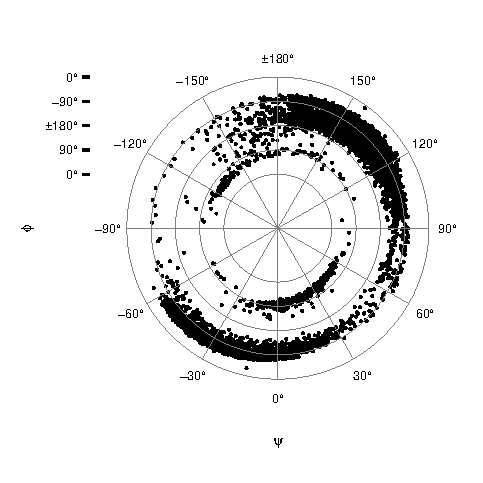
\includegraphics{torsion}
\end{center}
\caption{Polar plot of randomly sampled torsion angles}
\label{fig:torsion}
\end{figure}

\subsection{Linear Encoding of Protein Structure}

The polar plot described above is used to define torsion angle regions for each secondary structure assignment. 
The eight DSSP secondary structure assignment codes defined in \citet{Kabsch1983} divide into three groups in which torsion angle regions are roughly the same: `G',`H',`I', and `T' corresponding to $3_{10}$-helix, $\alpha$-helix, $\pi$-helix, and turn, respectively; `E' and `B' corresponding to $\beta$-strand and $\beta$-bridge, respectively; and `S' and `C' corresponding to bend and coil, respectively.

Polar plots for each group of DSSP assignment codes along with defined regions and descriptor designations are shown in \figurename~\ref{fig:torsion_refs}, with the exception of turns and bridges, which receive descriptors 11 and 12, respectively. 
For each polar plot, there are well-defined continuous regions of torsion angles that remain continuous in the plots. 
The only exception is found in the bends and coil plot at $\psi = 60\degree$ between $\phi = -180\degree$ and $\phi = 0\degree$.

%\begin{figure}[t]
%\begin{center}
%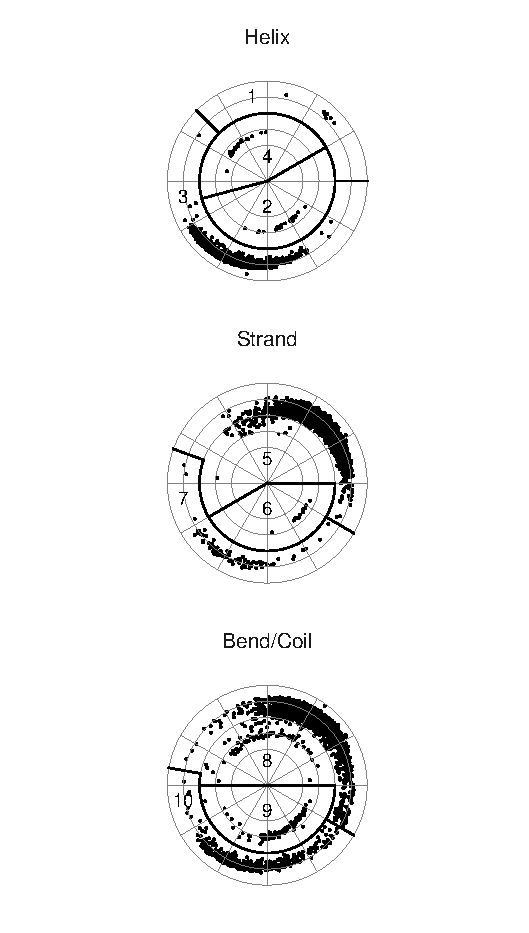
\includegraphics{torsion_refs}
%\end{center}
%\caption{Polar plots of randomly sampled torsion angles with designated descriptors for region and DSSP code combinations}
%\label{fig:torsion_refs}
%\end{figure}

\tablename~\ref{tab:codes} summarizes the mapping between region and secondary structure assignment combinations and ranges of integer valued descriptors.  
The specific mapping was arrived at primarily based on quality of results. 

\begin{table}[!t]
    \caption{DSSP Code/Descriptor Map}
    \label{tab:codes}
\centering
\begin{tabular}{lll}
\toprule
    \head{DSSP Codes} & \head{SS} & \head{Descriptors}\\
\midrule
    G, H, I & helix & 1-4\\
    E & strand & 5-7\\
    S, C & bend, coil & 8-10\\
    T & turn & 11\\
    B & bridge & 12\\
\bottomrule
\end{tabular}
\end{table}

Our initial use of Ramachandran plots to identify regions resulted in the frequent case of highly similar domains from the same CATH s95 clusters being considered significantly different. 
Alignment of these domains in PyMOL \citep{PyMOL} and the development of a script to label residues with their descriptors showed that slight differences in structure often resulted in distinct descriptors being assigned to aligned residues. 
Once we defined regions using the less confusing polar plots, this discrepancy was no longer observed. 

As an example of our linear encoding, the following sequence of descriptors represents a $\beta$-turn-$\beta$ motif followed by bends and coil.
\begin{gather}\label{E:descrseq} 
    [\, 5, 5, 5, 5, 5, 11, 11, 5, 5, 5, 5, 5, 8, 8, 10, 9 \,]
\end{gather}

Secondary structure assignments for termini are not always consistent among the variety of secondary structure assignment tools \citep{Martin2005}. 
We also observed this to be the case for DSSP assignments across homologous domains. 
Here, we introduce a heuristic we call \emph{secondary structure extension} (SSE) to address this variance. 

SSE iterates a sequence of descriptors once in both the forward and backward directions. 
Whenever a helix or strand descriptor is encountered, the next descriptor receives the same assignment as the preceding residue if its torsion angles match the region of the preceding residue, regardless of its own secondary structure assignment. 

SSE performed on the sequence found in (\ref{E:descrseq}) gives the sequence in (\ref{E:extdescrseq}).
Notice, the subsequence $[\, 8, 8 \,]$ in (\ref{E:descrseq}), corresponding to bends with torsion angles falling in the densest region of $\beta$-strand residues, becomes $[\, 5, 5 \,]$ in (\ref{E:extdescrseq}). 
\begin{gather}\label{E:extdescrseq} 
    [\, 5, 5, 5, 5, 5, 11, 11, 5, 5, 5, 5, 5, 5, 5, 10, 9 \,]
\end{gather}

Though \citet{Martin2005} lends some support to this heuristic, we use it primarily based on its performance. 

\subsection{Bag representation of protein structure}

Once a linear encoding for a protein structure is obtained, it needs to be further transformed into a representation suitable for fast and scalable similarity comparisons to other structures.
The processing of text documents within Information Retrieval~(IR) has long been used to satisfy these requirements using bag representations.
There are two distinct categories of representations for documents, syntactic and semantic, and much of the research applying IR to protein structure search has focused on the latter \citep{Aungand2004,Zhang2010,Budowski2010}. 

We have adapted the syntactic approach to document similarity, often referred to as shingling \citep{Broder1997a}, to our linear encoding of protein structure. 
We transform a linear sequence of descriptors into a multiset of shingles consisting of 4 consecutive descriptors.
The overlap between shingles ensures some of the order information within the original sequence is preserved in the bag. 

By shingling, we obtain a multiset of ordered lists from an ordered list of numbers. 
As an example, the sequence in (\ref{E:extdescrseq}) is transformed into the following bag of shingles. 
\begin{align}\label{E:shinglebag}
    \begin{split}
    \{\,&[5, 5, 5, 5], [5, 5, 5, 5], [5, 5, 5, 11], [5, 5, 11, 11], \\
        & [5, 11, 11, 5], [11, 11, 5, 5], [11, 5, 5, 5], [5, 5, 5, 5], \\
        & [5, 5, 5, 5], [5, 5, 5, 5], [5, 5, 5, 5], [5, 5, 5, 10], \\
        & [5, 5, 10, 9] \,\}
    \end{split}
\end{align}

Next, each shingle $s$ is hashed to an integer as shown in~(\ref{E:hashdef}). 
The hash function used is a simplification of the hash function used in the Rabin-Karp algorithm \citep{Karp1987}.
The prime number $13$ is used as the base since it is large enough to spread the descriptor values out in hash space without collisions. 
\begin{gather}\label{E:hashdef}
    s_{hash} = s_1 \times 13^3 + s_2 \times 13^2 + s_3 \times 13 + s_4
\end{gather}
Subsequently, the multiset in (\ref{E:shinglebag}) becomes the following bag of integers.
\begin{align}\label{E:hashbag}
    \begin{split}
    \{\,&11900, 11900, 11906, 11984, 12992, \\
        &26096, 25082, 11900, 11900, 11900, \\
        &11900, 11905, 11969 \,\}
    \end{split}
\end{align}

This final step completes the transformation of an ordered list of descriptors to a multiset of integers that still retains some of the order information present in the original list. 

Notice in (\ref{E:hashbag}) the value 11900, corresponding to the shingle $[ 5, 5, 5, 5 ]$, occurs frequently indicating the presence of a $\beta$-strand. 
Since most proteins are dominated by regular secondary structure, the abundance of shingles for $\beta$-strands as well as the three types of helices, end up dominating comparisons. 
Moreover, since shingles are limited in length, this situation allows for structures with many short $\beta$-strands to match structures with fewer long $\beta$-strands.
The same situation applies to helices. 

To address this lack of specificity, we introduce a heuristic we call \emph{run position encoding} (RPE). 
To distinguish between short and long runs, thereby increasing the specificity of the shingles, we add a factor of $10^5$ to each shingle hash as a function of the first residue's position in a run $i$. 
\begin{gather}
    runfactor(i) = 
    \begin{cases}
        i               &\text{if $i < \lfloor l/2 \rfloor$}\\
        l - i - 1       &\text{otherwise} 
    \end{cases}
\end{gather}
where $i$ is zero-based and $l$ is the length of the run. 
Multiplying by $10^5$ places the run factor as the left-most digit in the hash to avoid interference with the digits provided by the hash in (\ref{E:hashdef}).
This placement is also convenient for visual inspection, since the run factor is isolated as the left-most digit. 

The run factors for the sequence in (\ref{E:extdescrseq}) are
\begin{align}
    [\, 0, 1, 2, 1, 0, 0, 0, 0, 1, 2, 3, 2, 1, 0, 0, 0 \,].
\end{align}
Applied to the bag of integers in (\ref{E:hashbag}) gives
\begin{align}\label{E:rpebag}
    \begin{split}
    \{\,&011900, 111900, 211906, 111984, 012992, \\
        &026096, 025082, 011900, 111900, 211900, \\
        &311900, 211905, 111969 \,\},
    \end{split}
\end{align}
where the leading zero run factors are shown for clarity. 

This pyramidal approach preserves matches at the boundaries between secondary structure runs and loops that would not otherwise be preserved in the presence of differences in run lengths of one or more. 

To see why RPE run factors are calculated at the descriptor level and factored in at the shingle level, consider shingling a list of RPE run factors themselves, which mirrors applying them at the descriptor level. 
\begin{align*}
    &\text{The sequence of RPE factors} \\
    &\qquad[\, 0, 1, 2, 3, 2, 1, 0 \,] \text{ becomes} \\
    &\qquad\{\, [0, 1, 2, 3], [1, 2, 3, 2], [2, 3, 2, 1], [3, 2, 1, 0] \,\} \\
    &\text{and with one less element} \\
    &\qquad[\, 0, 1, 2, 2, 1, 0 \,] \text{ becomes} \\
    &\qquad\{\, [0, 1, 2, 2], [1, 2, 2, 1], [2, 2, 1, 0] \,\}
\end{align*}
Notice above, there is not a single shingle match for this one-off difference in run length.
Now consider shingling a list of RPE factors, but this time all elements in the shingle are set equal to the first element in the shingle, which mirrors applying them at the shingle level. 
\begin{align*}
    &\text{The sequence of RPE factors} \\
    &\qquad[\, 0, 1, 2, 3, 2, 1, 0 \,] \text{ becomes} \\
    &\qquad\{\, [0, 0, 0, 0], [1, 1, 1, 1], [2, 2, 2, 2], [3, 3, 3, 3] \,\} \\
    &\text{and with one less element} \\
    &\qquad[\, 0, 1, 2, 2, 1, 0 \,] \text{ becomes} \\
    &\qquad\{\, [0, 0, 0, 0], [1, 1, 1, 1], [2, 2, 2, 2] \,\}
\end{align*}
In this latter case, a one-off difference in run length results in one less shingle match while still serving to increase the specificity of the shingles. 

Now that we have a representation of a protein structure as a bag of integers, similarity between any two structures $a$ and $b$ is defined as the Jaccard similarity \citep{Levan1971} for multisets,
\begin{align}
    J(a,b) = \frac{\sum_i min(a_i, b_i)}{\sum_i max(a_i,b_i)}\text{,}
\end{align}
where $i$ ranges over all possible shingle hashes $s_i$ and $a_i$ and $b_i$ give the counts of shingle hash $s_i$ in structures $a$ and $b$, respectively. 

\subsection{Fast and scalable structure search}

In IR, the bag of shingles representation of documents is used in the near dupe clustering of documents \citep{Broder1997b}.
One application of near dupe clustering is in the review stage of Electronic-Discovery \citep{Joshi2008}, which is the most expensive stage in a discovery process. 
Often millions of documents must be examined by a staff of attorneys to make a reasonable effort at providing all documents relevant to the discovery request. 
Grouping documents into near dupe clusters and assigning all documents within a cluster to a single reviewer reduces duplication of effort. 

In the case of near dupe clustering, each document must be compared to every other document in the collection, taking quadratic time.
For this task, min-hashing \citep{Broder1998} and locality sensitive hashing (LSH) \citep{Indyk1998} can be combined to reduce this to subquadratic time. 
Although we do not near dupe cluster domains, we can still leverage the techniques of min-hashing and LSH to speed up protein structure search by a large constant factor.

Min-hashing is used to randomly select items from a set of items by repeatedly randomly hashing the items, sorting the hashes into a list, and then selecting the minimum item in each permuted list.
If the same random permutation of items is performed on each set of items in a collection, the key result is that the probability of matching min-hashes is equal to the Jaccard similarity \citep{Broder1998}.
In order to approximate the Jaccard similarity for a given pair of sets, a sufficient number of min-hashes must be obtained. 

In our case, the items are bags of shingle hashes for protein structures from which we obtain 60 min-hashes as described in \citet{Rajaraman2012}. 
Given the key result above, the Jaccard similarity can now be approximated by the proportion of matching min-hashes. 

Weighted min-hashing \citep{Chum2008} with integral weights is an extension to min-hashing that can be applied to multisets where the frequency of a hash within a multiset is used as its weight. 

Next, we use the LSH banding technique as described in \citet{Rajaraman2012}.
The key result of the banding technique is that if \emph{any} band positions are a match for a given pair of structures, the probability that a specific similarity threshold has been met can be calculated. 
We use 20 bands of 3-min-hashes where the probability of a Jaccard similarity of 60\% or greater is approximately 99\%. 
Banding allows the problem of finding similar items to be parallelized across bands since all that is needed for a match is a single band match. 

Together, min-hashing and LSH allow for a fast and scalable protein structure search using run position encoded shingles of residue descriptors.  

\section{RESULTS}

\subsection{Results subsection one}

Text. Text. Text. Text. Text. Text. Text. Text. Text. Text. Text.
Text. Text. Text. Text. Text. Text. Text. Text. Text. Text. Text.
Text. Text. Text. Text. Text. Text. Text. Text. Text. Text. Text.
Text. Text. Text. Text. Text. Text. Text. Text. Text. Text. Text.
Text. Text. Text. Text. Text. Text. Text. Text. Text. Text. Text.
Text. Text. Text. Text. Text. Text. Text. Text. Text. Text. Text.
Text. Text. Text. Text. Text. Text. Text. Text. Text. Text. Text.
Text. Text. Text. Text. Text. Text. Text. Text. Text. Text. Text.
Text. Text. Text. Text. Text. Text. Text. Text. Text. Text. Text.
Text. Text. Text. Text. Text. Text. Text. Text. Text. Text. Text.
Text. Text. Text. Text. Text. Text. Text. Text. Text. Text. Text.
Text. Text. Text. Text. Text. Text. Text. Text. Text.

\subsection{Results subsection two}

Text. Text. Text. Text. Text. Text. Text. Text. Text. Text. Text.
Text. Text. Text. Text. Text. Text. Text. Text. Text. Text. Text.
Text. Text. Text. Text. Text. Text. Text. Text. Text. Text. Text.
Text. Text. Text. Text. Text. Text. Text. Text. Text. Text. Text.
Text. Text. Text. Text. Text. Text. Text. Text. Text. Text. Text.
Text. Text. Text. Text. Text. Text. Text. Text. Text. Text. Text.
Text. Text. Text. Text. Text. Text. Text. Text. Text. Text. Text.
Text. Text. Text. Text. Text. Text. Text. Text. Text. Text. Text.
Text. Text. Text. Text. Text. Text. Text. Text. Text. Text. Text.
Text. Text. Text. Text. Text. Text. Text. Text. Text. Text. Text.
Text. Text. Text.

\section{CONCLUSION}

Text. Text. Text. Text. Text. Text. Text. Text. Text. Text. Text.
Text. Text. Text. Text. Text. Text. Text. Text. Text. Text. Text.
Text. Text. Text. Text. Text. Text. Text. Text. Text. Text. Text.
Text. Text. Text. Text. Text. Text. Text. Text. Text. Text. Text.
Text. Text. Text. Text. Text. Text. Text. Text. Text. Text. Text.
Text. Text. Text. Text. Text. Text. Text. Text. Text. Text. Text.
Text. Text. Text. Text. Text. Text. Text. Text. Text. Text. Text.
Text. Text. Text. Text. Text. Text. Text. Text. Text. Text. Text.
Text. Text. Text. Text. Text. Text. Text. Text. Text. Text. Text.
Text. Text. Text.

\subsubsection{Conflict of interest statement.} None declared.
\newpage

\nocite{Ayoub2017}
\nocite{BioJava2012}
\bibliography{rupee}
\bibliographystyle{NAR-natbib}

\end{document}
